
\subsection{Compiler}

In this section, we describe the compilation of EDMA data definition
files. The compiler consists of three parts: a parser, a translator,
and a generator. An overview of the compilation process can be seen
on Figure~\ref{fig:compilation}.

\begin{figure}[h]
	\centering
	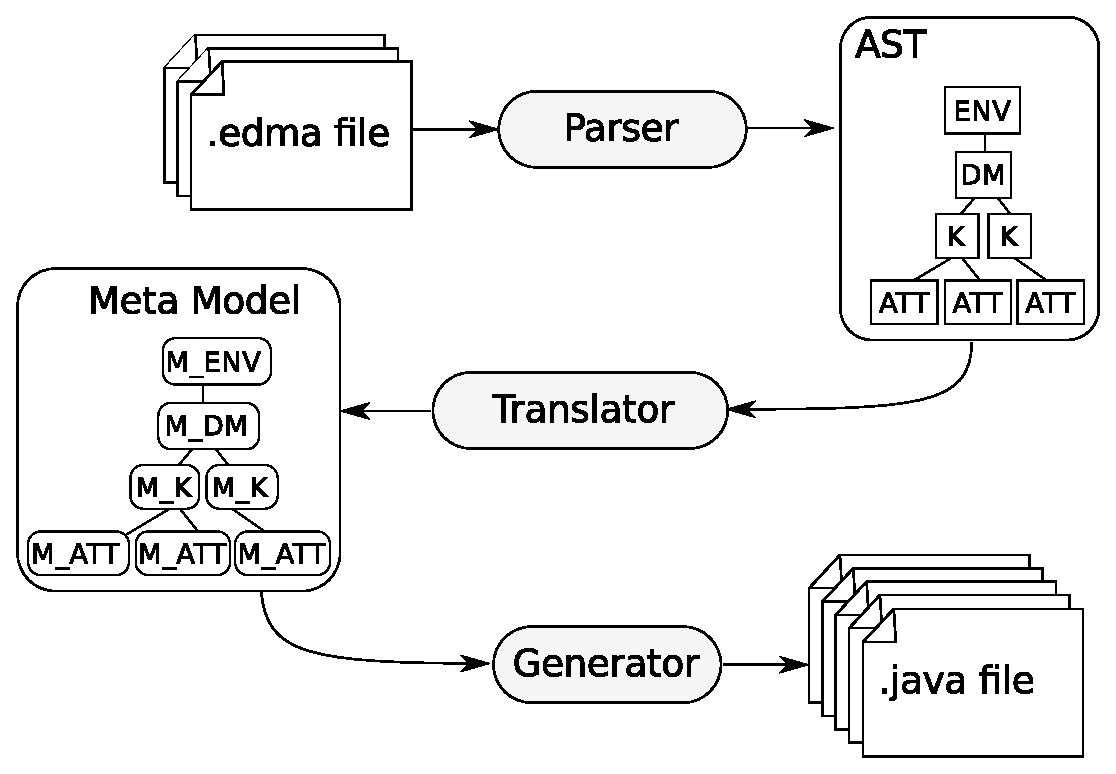
\includegraphics[scale=0.5]{img/compilation.pdf}
	\caption{The compilation of EDMA data definition files is done in three steps: parsing, compilation into a meta model, and generation of Java files.}
	\label{fig:compilation}
\end{figure}

A parser takes in one or many data model definition files with the
extension \texttt{.edma}. While parsing the files, an abstract syntax
tree (AST) representing the data models, is being created. The translator
translates the AST into a meta model, which can then be fed to the
generator. The generator is responsible for outputting Java classes
and interfaces, reflecting the user's data model definition.

It is worth noting, that the abstract syntax tree defines the logical
structure of our environment and data models. The important feature
of the AST is that it makes the translator completely independent
of the concrete textual syntax used in the EDMA language. Having the
AST makes it easy to change the textual grammar and create other syntaxes,
and even create other types of syntaxes. For example, it would be
possible to implement a graphical user interface for drawing data
models, thus serving as a syntax.


\subsubsection{Parser}

For defining the grammer of the textual syntax, we have used a parser
/ scanner generator known as JavaCC. From a JavaCC-grammer, a Java-based
top-down LL(k) parser is generated. The grammar specification is a
variation of EBNF, mixed with Java code for building an instance of
the AST.


\subsubsection{Translator}

The translator takes an AST representing the data model definition,
and creates a meta model instance. The meta model instance can be
seen as an internal representation of the data model definition, and
it is used by both the generator, and by the EDMA runtime system.

When the translator has got a complete AST from the parser, resembling
the user's data model, it does two things. First, it checks whether
everything is consistent within the AST. Then, it simply translates
the AST instance into a Meta Model instance.


\subparagraph{AST Consistency}

In the grammar, syntactical rules governing the data model definition
are specified. However, even if the language is only a data definition
language, there are also some semantic rules, that we must enforce.
Before translating the AST into a meta model, the translator checks
for the presence of circular extensions, unknown references, invalid
ranges in constraints, and value domain loops.
\begin{description}
\item [{Circular~Extensions}] -- The kinds Person and Student could be
defined to extend each other. Instantiation of either would require
an instance of the other to exist. Therefore, we prohibit the user
from making circular extensions of kinds.
\item [{Unknown~References}] -- Wherever the user has written a reference
to an attribute name or a kind name, it must be checked whether the
given attribute or kind is actually defined.
\item [{Value~Domain~Range~Checks}] -- Since the user can specify ranges
on numerical value domains, we have to check that the ranges supplied
actually make sense. For example having a minimum value that is greater
than the maximum value, should be invalid.
\item [{Value~Domain~Loops}] -- Having immutable value domains may be
tricky for the unaware user. Without any check for loops, the user
would be able to define value domains for which there could never
be a valid value. A value domain A of type Struct, could contain an
attribute b, of type \texttt{B}. Likewise, a value domain B of type
Struct could contain an attribute of type A. This is shown on the
listing below.\\
\begin{lstlisting}
ValueDomain A : Struct {
  b : B
}
ValueDomain B : Struct {
  a : A
}
\end{lstlisting}Since in A, b is not optional, it must be supplied at the instantiation
of A. Similarly, when creating a value of B, a value of A must be
supplied. The user could declare a type of B, and set it to null,
and feed it to A upon creation, but this will make the instantiation
of B fail with a nullpointer exception. Since the user might accidentially
create loops, by having many different inter-related value domains,
we have put a check into the compiler, to make it fail as early as
possible.
\end{description}
As soon as an error has been found in the AST, we print out the problem,
the file name and the line number where the error occurred. Each element
in the AST is created with the file name and line number of the statement,
that was the source of it's creation. Therefore, we can easily print
it out when an error occurs in the compilation stage.

After the meta model has been created, the compiler invokes the Generator,
which then starts generating the model-specific Java code.
